\chapter{基本原理:解决泊松方程}
\label{ch:fundamentals}

\begin{summary}
本章的目标是展示泊松方程如何
所有 PDE 中最基本的都可以用几行快速解决
的 FEniCS 代码。 我们介绍最多
基本 FEniCS 对象:
\texttt{Mesh}, \texttt{Function}, \texttt{FunctionSpace}, \texttt{TrialFunction}, \texttt{TestFunction}。
了解如何编写基本的 PDE 求解器,
包括如何制定数学变分问题,
应用边界条件,调用 FEniCS 求解器和绘图
解决方案。
\end{summary}


\section{数学问题的制定}
\label{ftut:poisson1:bvp}
\index{Poisson's equation}

许多关于编程语言的书籍都以HelloWorld开头
程序。 读者好奇知道基本的任务是什么
用语言表达,并将文字打印到屏幕上即可
这样的一个任务。 在有限元方法的世界,PDE,
最基本的任务是解决泊松方程。 我们的
因此对应于古典HelloWorld程序
解决以下边界值问题:

\begin{alignat}{2}
- \nabla^2 u(\x) &= f(\x),\quad &&\x\mbox{ in } \Omega,
\label{ftut:poisson1}\\
u(\x) &= \ub(\x),\quad &&\x\mbox{ on } \partial \Omega\tp \label{ch:poisson0:bc}
\end{alignat}

这里,$u = u(\x)$是未知函数,$f = f(\x)$是
规定的函数,$\nabla^2$是Laplace算子
(通常写为$\Delta$),$\Omega$是空间域,而
$\partial \Omega$是$\Omega$的边界。 Poisson问题,
包括PDE $-\nabla^2u = f$和边界条件
$u = \ub$ on $\partial \Omega$,是边界值的一个例子
问题,必须在之前精确地陈述
使用FEniCS开始解决它是有意义的。

在具有坐标$x$和$y$的两个空间维度中,我们可以写出来
Poisson方程为

\begin{equation}
- {\partial^2 u\over\partial x^2} -
{\partial^2 u\over\partial y^2} = f(x,y)\tp
\end{equation}

未知的$u$现在是两个变量$u = u(x,y)$的函数
在二维域$\Omega$。

Poisson方程出现在许多物理环境中,包括
热传导,静电,物质扩散,扭转
弹性棒,非粘性流体流和水波。 而且,
方程出现在数值分割策略中更为复杂
PDE系统,特别是Navier-Stokes方程。

解决边界值问题,如Poisson方程
FEniCS包括以下步骤:

\begin{enumerate}
\item 识别计算域($\Omega$),PDE,它 边界条件和源项($f$)。
\item 将PDE重新定义为有限元变分问题。
\item 编写一个定义计算域的Python程序,变分问题,边界条件和来源
  条款,使用相应的FEniCS抽象。
\item 调用FEniCS来解决边界值问题,并且可选地,扩展程序
计算衍生量,如通量和平均值,以及 可视化结果。
\end{enumerate}

\noindent
现在我们将详细介绍第2--4步。 的主要特点
FEniCS是步骤3和4导致相当短的代码,而a
大多数其他PDE软件框架中的类似程序都需要
更多的代码和技术上困难的编程。

\begin{notice}[什么使FEniCS有吸引力?]
虽然许多软件框架都非常优雅
HelloWorld 的例子
Poisson方程式,FEniCS是我们知道的唯一框架
代码保持紧凑和美观,非常接近数学
即使是数学和算法的复杂性
从笔记本电脑转移到高性能时会增加
计算服务器(集群)。
\end{notice}

\subsection{有限元变分法}
\label{ch:poisson0:varform}
\index{variational formulation}

FEniCS是基于有限元法,它是一般的和
高效数学机械的数值解
PDE。 有限元方法的出发点是PDE
以变体形式表达。 不熟悉的读者
变数问题将会简要介绍一下这个话题
在本教程中,但阅读有限元上的正确书
鼓励方法。 经验表明,您可以使用
FEniCS作为解决PDE的工具,即使没有深入的了解
有限元法,只要你有人帮你
将PDE作为变分问题。

\index{test function}
\index{trial function}

将PDE转化为变分问题的基本方法是
将PDE乘以函数$v$,整合得到的等式
通过域$\Omega$,并按部分条款执行整合
与二阶导数。 函数$v$乘以
PDE称为测试功能。 未知函数$u$为
近似被称为试验函数。 试用版和
测试功能也用于FEniCS程序。 试用和测试
功能属于指定的所谓功能空间
功能的属性。

\index{integration by parts}

在这种情况下,我们先乘以Poisson方程
通过测试函数$v$并集成$\Omega$:

\begin{equation}
\label{ch:poisson0:multbyv}
-\int_\Omega (\nabla^2 u)v \dx = \int_\Omega fv \dx\tp
\end{equation}
我们这里让$\dx$表示用于集成的差分元素
域$\Omega$。 我们稍后会让$\ds$表示差分
在$\Omega$的边界上整合的元素。

当我们得出变分公式时,一个常见的规则就是我们尝试
保持$u$和$v$的衍生工具的顺序尽可能小
可能。 在这里,我们有一个$u$的二阶空间导数,
这可以转换为$u$和$v$的一阶导数
应用零件整合技术。 公式
读

\begin{equation}
\label{ch:poisson0:eqbyparts}
 -\int_\Omega (\nabla^2 u)v \dx
= \int_\Omega\nabla u\cdot\nabla v \dx - \int_{\partial\Omega}{\partial u\over
\partial n}v \ds,
\end{equation}

其中$\frac{\partial u}{\partial n} = \nabla u \cdot n$是
$u$的衍生物向外向正方向$n$
边界。

变分配方的另一个特点是
测试函数$v$需要在部分消失
解决方案$u$的边界已知。
在现在
问题,这意味着$v = 0$在整个边界$\partial \Omega$。
第二个术语在右边
(\ref{ch:poisson0:eqbyparts})因此消失。 从
(\ref{ch:poisson0:multbyv})和(\ref{ch:poisson0:eqbyparts})
遵循

\begin{equation}
\int_\Omega\nabla u\cdot\nabla v \dx = \int_\Omega fv \dx\tp
\label{ch:poisson0:weak1}
\end{equation}

如果我们要求该方程适用于所有测试函数$v$
一些合适的空间$\hat V$,所谓的测试空间,我们获得一个
明确的数学问题,唯一地决定了
解决方案$u$在于一些可能不同的功能空间
$V$,所谓的试验空间。 我们参考
(\ref{ch:poisson0:weak1})作为弱形式或变体形式
原边界值问题
(\ref{ftut:poisson1})--(\ref{ch:poisson0:bc})。

适当的陈述
我们的变分问题现在如下:
找到$u \in V$这样

\begin{equation} \label{ch:poisson0:var}
  \int_{\Omega} \nabla u \cdot \nabla v \dx =
  \int_{\Omega} fv \dx
  \quad \forall v \in \hat{V}\tp
\end{equation}

现在试用和测试空间$V$和$\hat V$
问题定义为

\begin{align*}
     V      &= \{v \in H^1(\Omega) : v = \ub \mbox{ on } \partial\Omega\}, \\
    \hat{V} &= \{v \in H^1(\Omega) : v = 0 \mbox{ on } \partial\Omega\}\tp
\end{align*}
简而言之,$H^1(\Omega)$是数学上众所周知的Sobolev空间
包含函数$v$,使$v^2$和$|\nabla v|^2$有
有限积分超过$\Omega$(基本上意味着函数
是连续的)。 底层PDE的解决方案必须在于
函数空间中的衍生物也是连续的,但是
Sobolev空间$H^1(\Omega)$允许不连续的函数
衍生物。 $u$的连续性要求较弱
变量语句(\ref{ch:poisson0:var}),作为结果
整合部分,具有很大的实际后果
构造有限元函数空间。 特别是它
允许使用分段多项式函数空间; 即功能
通过简单地将多项式函数拼接在一起构成的空间
域,如间隔,三角形或四面体。

变量问题(\ref{ch:poisson0:var})是连续的
问题:它定义了无穷维的解$u$
功能空间$V$。 Poisson方程的有限元法
找出变分问题的近似解
(\ref{ch:poisson0:var})替换无限维函数
空间$V$和$\hat{V}$通过离散(有限维)试验
测试空间$V_h\subset{V}$和$\hat{V}_h\subset\hat{V}$。 离散变分问题如下:
找到$u_h \in V_h \subset V$这样

\begin{equation} \label{ch:poisson0:vard}
  \int_{\Omega} \nabla u_h \cdot \nabla v \dx =
  \int_{\Omega} fv \dx
  \quad \forall v \in \hat{V}_h \subset \hat{V}\tp
\end{equation}

这个变分问题,连同一个合适的定义
函数空间$V_h$和$\hat{V}_h$,唯一地定义我们的近似值
Poisson方程的数值解(\ref{ftut:poisson1})。 注意
边界条件被编码为试验和测试的一部分
空间。 起初,数学框架可能看起来很复杂
一瞥,但好消息是有限元变分
问题(\ref{ch:poisson0:vard})看起来和连续的一样
变分问题(\ref{ch:poisson0:var})和FEniCS可以
自动解决变量问题,如(\ref{ch:poisson0:vard})!

\begin{notice}[我们的意思是符号$u$和$V$]
关于变数问题的数学文献写了$u_h$
解的离散问题和$u$的解决方案
连续问题 获得(几乎)一对一的关系
在一个问题的数学表达与之间
相应的FEniCS程序,我们将下拉$_h$和使用
$u$用于解决离散问题。
我们将使用$\uex$来确定
解决连续问题,如果我们需要明确区分
两者之间。 类似地,我们将让$V$表示离散有限
元素功能空间,我们寻求我们的解决方案。
\end{notice}

\subsection{抽象有限元变分公式}
\label{ch:poisson0:abstrat}
\index{abstract variational formulation}

原来是方便的介绍下列规范
变量问题的符号:找到$u \in V$这样

\begin{equation}
a(u, v) = L(v) \quad \forall v \in \hat{V}.
\end{equation}

对于Poisson方程,我们有:

\begin{align}
a(u, v) &= \int_{\Omega} \nabla u \cdot \nabla v \dx,
\label{ch:poisson0:vard:a}\\
L(v) &= \int_{\Omega} fv \dx\tp  \label{ch:poisson0:vard:L}
\end{align}

从数学文献中,$a(u,v)$被称为双线性
形式和$L(v)$作为线性形式。 我们将在每一个线性问题中
我们解决,确定与未知$u$的条款并收集他们
$a(u,v)$,并且类似地收集只有已知功能的所有术语
$L(V)$。 $a$和$L$的公式可以直接表达
我们的FEniCS计划。

为了解决FEniCS中的线性PDE,如Poisson方程,用户
因此需要执行两个步骤:

\begin{itemize}
\item 通过指定选择有限元空间$V$和$\hat V$
域(网格)和函数空间的类型(多项式)
度和类型)。
\item 将PDE表示为(离散)变分问题:找到$u\in V$
所以$a(u,v) = L(v)$为$v\in \hat{V}$。
\end{itemize}

\noindent
\subsection{选择测试问题}
\label{ch:poisson0:testproblem}

泊松问题 (\ref{ftut:poisson1})--(\ref{ch:poisson0:bc})有
远程功能一般域$\Omega$和一般功能$\ub$
边界条件和右边的$f$。 对于我们的第一个
实现我们将需要为$\Omega$做出具体的选择,
$\ub$和$f$。 构建一个已知的问题是明智的
分析解决方案,使我们可以方便地检查计算
解决方案是正确的。 低阶多项式的解是
主要候选人 标准有限元函数空间的度数
$r$将完全重现度为$r$的多项式。 分段
线性元素($r = 1$)能够精确地再现二次方
均匀分布网格上的多项式。 这个重要的结果可以
用于验证我们的实现。 我们只是制造一些
比如说2D中的二次函数作为确切的解决方案

\index{test problem}

\begin{equation}
\label{ch:poisson0:impl:uex}
\uex(x,y) = 1 +x^2 + 2y^2\tp
\end{equation}

通过将(\ref{ch:poisson0:impl:uex})插入到Poisson方程式中
(\ref{ftut:poisson1}),我们发现$\uex(x,y)$是一个解决方案,以便

\[ f(x,y) = -6,\quad \ub(x,y)=\uex(x,y)=1 + x^2 + 2y^2,\]
只要$\uex$被规定,不管域的形状
边界。 我们在这里选择,为了简单,
该域为单位广场,

\[ \Omega = [0,1]\times [0,1] \tp\]
这个简单但非常强大的构建测试问题的方法是
称为制造解决方案:选择一个简单
表达式为精确解,将其插入等式获得
右边(源项$f$),然后用公式求解
这个右手边使用精确的解决方案作为边界
条件,并尝试重现确切的解决方案。

\index{verification}
\index{exact solution}
\index{method of manufactured solutions}

\begin{notice}[提示:尝试使用精确的数值解决方案验证您的代码!]
测试数值方法实现的常用方法
是比较数字
解决方案具有测试问题的精确解析解
得出结论,如果错误是“足够小”,该程序可以工作。
不幸的是,不可能知道一个大小为$10^{ - 5}$的错误
$20\times 20$ mesh的线性元素是预期的准确度
数值近似或者如果误差也包含a的影响
代码中的错误。我们通常都知道数值误差是它的
\emph{asymptotic properties},例如它与$h^2$成正比
如果$h$是网格中单元格的大小。然后我们比较
使用不同的$h$-values来查看网格的错误,看是否渐近
行为是正确的。这是一个非常强大的验证
技术,并在〜\ref{ch:poisson0:convrates}部分中详细解释。
但是,如果我们有一个测试问题
我们知道应该没有近似误差,我们知道
PDE问题的分析解决方案应该重现
机器精度由程序。这就是为什么我们强调这种
本教程中的测试问题。通常,元素
degree $r$可以重现度为$r$的多项式,所以这样
是构建无数值解的起点
近似误差
\end{notice}

\section{FEniCS实现}
\label{ch:poisson0:impl}

\subsection{完整的程序}
一个用于解决Poisson方程的测试问题的FEniCS程序
在2D中,给定的$\Omega$,$\ub$和$f$的选项可能看起来像
如下:

\begin{python}
from fenics import *

# Create mesh and define function space
mesh = UnitSquareMesh(8, 8)
V = FunctionSpace(mesh, 'P', 1)

# Define boundary condition
u_D = Expression('1 + x[0]*x[0] + 2*x[1]*x[1]', degree=2)

def boundary(x, on_boundary):
    return on_boundary

bc = DirichletBC(V, u_D, boundary)

# Define variational problem
u = TrialFunction(V)
v = TestFunction(V)
f = Constant(-6.0)
a = dot(grad(u), grad(v))*dx
L = f*v*dx

# Compute solution
u = Function(V)
solve(a == L, u, bc)

# Plot solution and mesh
plot(u)
plot(mesh)

# Save solution to file in VTK format
vtkfile = File('poisson/solution.pvd')
vtkfile << u

# Compute error in L2 norm
error_L2 = errornorm(u_D, u, 'L2')

# Compute maximum error at vertices
vertex_values_u_D = u_D.compute_vertex_values(mesh)
vertex_values_u = u.compute_vertex_values(mesh)
import numpy as np
error_max = np.max(np.abs(vertex_values_u_D - vertex_values_u))

# Print errors
print('error_L2  =', error_L2)
print('error_max =', error_max)

# Hold plot
interactive()
\end{python}

该示例程序可以在文件中找到{\nolinkurl{ft01_poisson.py}}。
\begin{center}
  \url{https://fenicsproject.org/pub/tutorial/python/vol1/ft01_poisson.py}
\end{center}

\index{ft01\_poisson.py@{\rm\texttt{ft01\_poisson.py}}}

\subsection{运行程序}
\label{ch:poisson0:impl:run}

FEniCS程序必须以纯文本文件的形式提供
文本编辑器,如Atom,Sublime Text,Emacs,Vim等。
有几种方法可以运行Python程序{\nolinkurl{ft01_poisson.py}}:
\begin{center}
  \url{https://fenicsproject.org/pub/tutorial/python/vol1/ft01_poisson.py}
\end{center}

\begin{itemize}
 \item 使用终端窗口。

 \item 使用集成开发环境(IDE),例如Spyder。

 \item 使用Jupyter笔记本。
\end{itemize}

\noindent
\paragraph{终端窗口。}
\index{terminal window}

打开一个终端
窗口,移动到包含程序的目录并键入
以下命令:

\begin{bash}
$ python ft01_poisson.py
\end{bash}

请注意,此命令必须在支持FEniCS的终端中运行。 对于
FEniCS Docker容器的用户,这意味着您必须键入
启动FEniCS会话后使用此命令
\texttt{fenicsproject run}或\texttt{fenicsproject start}。

运行上述命令时,FEniCS将运行程序进行计算
近似解$u$。 大概的解决方案$u$将是
与确切的解决方案$\uex = \ub$相比,$L^2$和
将打印最大规范。 既然我们知道我们的大概
解决方案应该在机器内重现精确的解决方案
精度,这个错误应该是小的,有的是顺序的
$10^{-15}$。 如果您的FEniCS安装中启用了绘图,
那么一个简单的解决方案的窗口将显示为
在图〜\ref{fig:poisson_plot}中。

\paragraph{Spyder。}
\index{Spyder}

许多人喜欢在一个集成的开发环境中工作
提供编程编辑器,执行代码的窗口,
用于检查对象的窗口等。只需打开文件
{\nolinkurl{ft01_poisson.py}}
\begin{center}
  \url{https://fenicsproject.org/pub/tutorial/python/vol1/ft01_poisson.py}
\end{center}
并按播放按钮运行它。 我们参考Spyder教程
了解更多关于在Spyder环境中工作的信息。 Spyder是
强烈推荐,如果你习惯在图形工作
MATLAB环境。

\paragraph{Jupyter notebooks。}
\index{Jupyter}

笔记本电脑可以将文本和可执行代码混合在一起
文档,但您也可以使用它来在网络中运行程序
浏览器。从终端窗口运行命令\texttt{jupyter notebook}
在GUI的右上角找到\textbf{New}下拉菜单,
在Python 2或3中选择一个新的notebook,写入\verb!%load ft01_poisson.py!在这个notebook的空白单元格中,然后按
Shift + Enter执行单元格。然后,将文件\nolinkurl{ft01_poisson.py}
\begin{center}
  \url{https://fenicsproject.org/pub/tutorial/python/vol1/ft01_poisson.py}
\end{center}
加载到
notebook。重新执行cell(Shift + Enter)运行程序。您
可以将整个程序划分成几个单元格进行检查
中间结果:将光标放在要分割的位置
cell并选择\textbf{Edit - Split Cell}。对于FEniCS Docker的用户
图像,运行\texttt{fenicsproject notebook}命令并按照
说明。要启用绘图,请确保运行该命令
\verb!%matplotlib inline!在notebook里面。

\section{解剖方案}
\label{ch:poisson0:impl:dissect}
我们现在将详细剖析我们的FEniCS计划。 列出的FEniCS
程序定义有限元网格,有限元函数空间
$V$在此网格上,边界条件为$u$(函数$\ub$),
和双线性和线性形式$a(u,v)$和$L(v)$。 此后,
解决方案$u$被计算。 在程序结束时,我们比较了
数值和确切的解决方案。 我们也使用该图来绘制解决方案
\texttt{plot}命令并将解决方案保存到外部文件
后期处理。

\subsection{重要的第一行}
程序的第一行,
\begin{python}
from fenics import *
\end{python}
导入关键类\texttt{UnitSquareMesh},\texttt{FunctionSpace},\texttt{Function},
等等,从FEniCS图书馆。 所有FEniCS程序
通过有限元法解决PDE通常从这开始
线。

\index{mesh}
\index{Mesh@{\rm\texttt{Mesh}}}

\subsection{生成简单的网格}
该声明
\begin{python}
mesh = UnitSquareMesh(8, 8)
\end{python}
在单位平方上定义均匀的有限元网格
$[0,1]\times [0,1]$。 网格由\emph{cells}组成,其中2D是三角形
有直边。 参数8和8指定正方形
应分为$8\times 8$矩形,每个分为一对
三角形。 三角形(cells)的总数因此变为
128。 网格中的顶点总数为$9\cdot 9=81$。
在后面的章节中,您将学习如何生成更复杂的网格。

\index{FunctionSpace@{\rm\texttt{FunctionSpace}}}
\index{finite element space}
\index{Lagrange finite element}
\index{P1 element}

\subsection{定义有限元函数空间}
\index{FunctionSpace@{\rm\texttt{FunctionSpace}}}
\index{function space}

一旦创建了网格,就可以创建一个有限元的功能空间
\texttt{V}:

\begin{python}
V = FunctionSpace(mesh, 'P', 1)
\end{python}

第二个参数\texttt{'P'}指定元素的类型。 的类型
这里的元素是$\mathsf{P}$,意味着标准的Lagrange系列
元素。 您也可以使用\texttt{'Lagrange'}来指定此类型
元件。 FEniCS支持所有单体元素族和符号
定义在\footnote{\texttt{https://www.femtable.org}}{有限元素周期表}\cite{ArnoldLogg2014}。
\begin{center}
  \url{https://www.femtable.org}
\end{center}

\index{Periodic Table of the Finite Elements}

第三个参数\texttt{1}指定有限元的程度。 在
这种情况下,标准的$\mathsf{P}_1$ linear xxzxLagrange元素,其中
是三角形,节点在三个顶点。 一些有限元
从业者将此元素称为“线性三角形”。该
计算的解决方案$u$将在元素和线性上是连续的
每个元素内的$x$和$y$变化。 高阶多项式
通过增加每个单元的近似值
\texttt{FunctionSpace}的第三个参数,然后生成函数
类型为$\mathsf{P}_2$,$\mathsf{P}_3$的空格等等。更改
\texttt{'DP'}的第二个参数创建一个函数空间
不连续的Galerkin方法。

\index{TestFunction@{\rm\texttt{TestFunction}}} \index{TrialFunction@{\rm\texttt{TrialFunction}}}
\index{DirichletBC@{\rm\texttt{DirichletBC}}}
\index{Dirichlet boundary conditions}

\subsection{定义试用和测试功能}
在数学中,我们区分试验空间$V$
和$\hat{V}$。 目前问题的唯一区别是
边界条件。 在FEniCS中,我们没有指定边界
条件作为功能空间的一部分,所以这是足够的工作
其中一个公共空间\texttt{V}用于试用和测试功能
程序:
\begin{python}
u = TrialFunction(V)
v = TestFunction(V)
\end{python}

\index{boundary specification (function)}

\subsection{定义边界条件}
下一步是指定边界条件:$u=\ub$ on
$\partial\Omega$。 这是完成的

\begin{python}
bc = DirichletBC(V, u_D, boundary)
\end{python}

\verb!u_D! 是定义解决方案值的表达式
boundary和\texttt{boundary}是定义的一个函数(或对象)
哪些点属于边界。

$u=\ub$类型的边界条件称为\emph{Dirichlet
条件}。 对于Poisson的当前有限元方法
问题,他们也被称为必需边界条件,因为它们
需要作为审判空间的一部分明确强加(相比之下)
被隐含地定义为变分公式的一部分)。
自然地,FEniCS类用于定义Dirichlet边界
条件命名为\texttt{DirichletBC}。

\index{Expression@{\rm\texttt{Expression}}}

变量\verb!u_D! 指的是一个\texttt{Expression}对象,用于
代表数学函数。 典型的建筑是

\begin{python}
u_D = Expression(formula, degree=1)
\end{python}

其中\emph{formula}是一个包含数学表达式的字符串。
公式必须用C ++语法编写
自动变成一个高效的,编译的C ++函数。

\begin{notice}[表达和准确性]
当定义一个\texttt{Expression}时,第二个参数\texttt{degree}是一个
指定应该如何处理表达式的参数
计算。 在每个本地元素上,FEniCS将内插
表达为有限元空间
的指定程度。 获得最佳
(顺序)计算的准确性,通常是一个很好的选择
使用与用于审判的空间$ V $相同的程度
和测试功能。 但是,如果使用\texttt{Expression}表示
一个精确的解决方案,用于评估计算的准确性
解决方案,更高的程度必须用于表达(一个或两个
度以上)。
\end{notice}

该表达式可能取决于变量\texttt{x[0]}和\texttt{x[1]}
对应于$x$和$y$坐标。 在3D中,表达式
也可能依赖于对应于$z$的变量\texttt{x[2]}
坐标。 我们选择$\ub(x,y)=1 + x^2 + 2y^2$,公式
字符串可以写为\texttt{1 + x[0]*x[0] + 2*x[1]*x[1]}:

\begin{python}
u_D = Expression('1 + x[0]*x[0] + 2*x[1]*x[1]', degree=2)
\end{python}

我们将学位设置为$2$,以便\verb!u_D! 可能代表确切的
二次解决我们的测试问题。

\index{C++ expression syntax}
\index{expression syntax (C++)}

\begin{notice}[字符串表达式必须具有有效的C++语法!]
\texttt{Expression}对象的字符串参数必须遵守C++语法。
数学表达式的大多数Python语法也是有效的C++语法,
但是权力表达式是一个例外:\texttt{p**a}必须写为
C++中的\texttt{pow(p, a)}(这也是一个替代的Python语法)。
以下数学函数可以直接使用
在C++中
定义\texttt{Expression}对象时的表达式:
\texttt{cos}, \texttt{sin}, \texttt{tan}, \texttt{acos}, \texttt{asin},
\texttt{atan}, \texttt{atan2}, \texttt{cosh}, \texttt{sinh}, \texttt{tanh}, \texttt{exp},
\texttt{frexp}, \texttt{ldexp}, \texttt{log}, \texttt{log10}, \texttt{modf},
\texttt{pow}, \texttt{sqrt}, \texttt{ceil}, \texttt{fabs}, \texttt{floor}, and \texttt{fmod}.
此外,数字$\pi$可用作符号\texttt{pi}。
所有列出的函数取自\texttt{cmath} C++头文件,和
因此可能
请参阅\texttt{cmath}的文档了解更多信息
各种功能。

If/else可以使用C语法进行内联分支。该
功能

\[ f(x,y) = \left\lbrace\begin{array}{ll} x^2, & x, y\geq 0,\\
2, & \hbox{otherwise},\end{array}\right.\]
被实现为

\begin{python}
f = Expression('x[0]>=0 && x[1]>=0 ? pow(x[0], 2) : 2', degree=2)
\end{python}

表达式字符串中的参数是允许的,但是
必须通过关键字初始化
创建\texttt{Expression}对象时的参数。 例如,
函数$f(x)=e^{-\kappa\pi^2t}\sin(\pi k x)$可以编码为

\begin{python}
f = Expression('exp(-kappa*pow(pi, 2)*t)*sin(pi*k*x[0])', degree=2,
               kappa=1.0, t=0, k=4)
\end{python}
随时可以更新参数:

\begin{python}
f.t += dt
f.k = 10
\end{python}
\end{notice}

\index{boundary specification (function)}

函数\texttt{boundary}指定属于哪些点
应用边界条件的边界的一部分:

\begin{python}
def boundary(x, on_boundary):
    return on_boundary
\end{python}
用于标记边界的\texttt{boundary}的函数必须返回
布尔值:\texttt{True}如果给定点\texttt{x}位于Dirichlet上
boundary和\texttt{False}否则。 参数\verb!on_boundary! 是\texttt{True}
如果\texttt{x}在网格的物理边界上,那么在现在
情况下,我们应该为所有的点返回\texttt{True}
边界,我们可以返回\verb!on_boundary!的提供值。该
将为每个离散点调用\texttt{boundary}函数
网格,这意味着我们可以定义$u$的边界
如果需要,在域内知道。

考虑FEniCS边界规范的一种方法是
FEniCS会问你(或者说是函数\texttt{boundary}哪个
你已经实现了)某个特定点\texttt{x}是否是其中的一部分
边界。 FEniCS已经知道该点是否属于
实际边界(域的数学边界)和善意
在变量\verb!on_boundary!中与您共享此信息。 您
可以选择使用这些信息(如我们在这里),或忽略它
完全。

参数\verb!on_boundary! 也可以省略,但在这种情况下,我们需要
测试\texttt{x}中的坐标值:

\begin{python}
def boundary(x):
    return x[0] == 0 or x[1] == 0 or x[0] == 1 or x[1] == 1
\end{python}

使用完全匹配测试比较浮点值
\texttt{==}不是很好的编程实践,因为小的舍入误差
在\texttt{x}值的计算中可以进行测试\texttt{x [0] == 1}
即使\texttt{x}位于边界上也变为虚假。 一个更好的考验是
明确地检查公平的公平

\begin{python}
tol = 1E-14
def boundary(x):
    return abs(x[0]) < tol or abs(x[1]) < tol \
        or abs(x[0] - 1) < tol or abs(x[1] - 1) < tol
\end{python}
或在FEniCS中使用\texttt{near}命令:

\begin{python}
def boundary(x):
    return near(x[0], 0, tol) or near(x[1], 0, tol) \
        or near(x[0], 1, tol) or near(x[1], 1, tol)
\end{python}

\index{tolerance}
\index{rounding errors}

\begin{notice}[不要使用\texttt{==}来比较实数!]
如果\texttt{x[0]}是真实的,则不应该使用像\texttt{x[0] == 1}的比较
number,因为\texttt{x[0]}中的舍入误差可能会使测试失败
当它在数学上是正确的。 考虑以下计算
在Python中:

\begin{python}
>>> 0.1 + 0.2 == 0.3
False
>>> 0.1 + 0.2
0.30000000000000004
\end{python}

需要使用公差进行实数比较!该
公差的值取决于所涉及的数字的大小
算术运算:

\begin{python}
>>> abs(0.1 + 0.2 - 0.3)
5.551115123125783e-17
>>> abs(1.1 + 1.2 - 2.3)
0.0
>>> abs(10.1 + 10.2 - 20.3)
3.552713678800501e-15
>>> abs(100.1 + 100.2 - 200.3)
0.0
>>> abs(1000.1 + 1000.2 - 2000.3)
2.2737367544323206e-13
>>> abs(10000.1 + 10000.2 - 20000.3)
3.637978807091713e-12
\end{python}
对于单位大小的数量,可以使用低至$3\cdot 10^{-16}$的公差
(实际上,这个容差在FEniCS中被称为常数\verb!DOLFIN_EPS!)。
否则,必须使用适当缩放的公差。
\end{notice}

\index{UFL}

\subsection{定义源术语}

在定义双线性和线性形式$a(u,v)$和$L(v)$ 之前
必须指定源术语$f$:

\begin{python}
f = Expression('-6', degree=0)
\end{python}
当$f$在域上是恒定的,\texttt{f}可以
更有效地表示为\texttt{Constant}:

\begin{python}
f = Constant(-6)
\end{python}

\subsection{定义变分问题}

我们现在有了我们需要定义的所有成分
变分问题:

\begin{python}
a = dot(grad(u), grad(v))*dx
L = f*v*dx
\end{python}
实质上,这两行指定要解决的PDE。 注意
Python语法之间非常接近的对应关系
数学公式$\nabla u\cdot\nabla v \dx$和$fv \dx$。 这个
是FEniCS的关键优势:变分中的公式
配方将直接转换为非常类似的Python代码,一个功能
这使得容易指定和解决复杂的PDE问题。该
用于表达弱表单的语言称为UFL (Unified Form Language)\cite{UFL_2014,FEniCS}
,并且是FEniCS的组成部分。

\begin{notice}[表达内在产品]
内部产品$\int_{\ Omega} \nabla u \cdot \nabla v \dx$
可以在FEniCS中以各种方式表达。 以上,我们用过
符号\texttt{dot(grad(u), grad(v))*dx}。 点产品在
FEniCS/UFL计算最后一个索引的总和(收缩)
的第一个因素和第二个因素的第一个指标。
在这种情况下,这两个因素都是一级(向量)和
所以这个总和刚刚超过$\nabla u$的一个单一的索引
和$\nabla v$。 计算矩阵的内积(与
两个索引),一个必须代替\texttt{dot}使用函数\texttt{inner}。
对于向量,\texttt{dot}和\texttt{inner}是等效的。
\end{notice}

\subsection{形成和求解线性系统}

定义了有限元变分问题和边界
条件下,我们现在可以要求FEniCS计算解决方案:

\begin{python}
u = Function(V)
solve(a == L, u, bc)
\end{python}

请注意,我们首先将变量\texttt{u}定义为\texttt{TrialFunction}和
用它来表示\texttt{a}中的未知数。 其后,我们
重新定义\texttt{u}成为表示解决方案的\texttt{Function}对象;
即计算的有限元函数$u$。 这个重新定义
变量\texttt{u}在Python中是可行的,通常用于FEniCS
线性问题的应用。 \texttt{u}的两种类型的对象
指的是从数学角度来看是相等的,因此是
对两个对象使用相同的变量名称是自然的。

\index{degrees of freedom}

\subsection{使用\texttt{plot}命令绘制解决方案}

\index{plotting}
\index{plot@{\rm\texttt{plot}}}

一旦解决方案被计算出来,它就可以被可视化
\texttt{plot}命令:

\begin{python}
plot(u)
plot(mesh)
interactive()
\end{python}
注意在\texttt{plot}命令之后调用函数\texttt{interactive}。
这个呼叫可以与地块(旋转和
变焦)。 对\texttt{interactive}的调用通常放在a的末尾
创建地块的程序。 Figure~\ref{fig:poisson_plot}显示
两个地块。

%\begin{figure}[!ht]  % fig:poisson_plot
%  \centerline{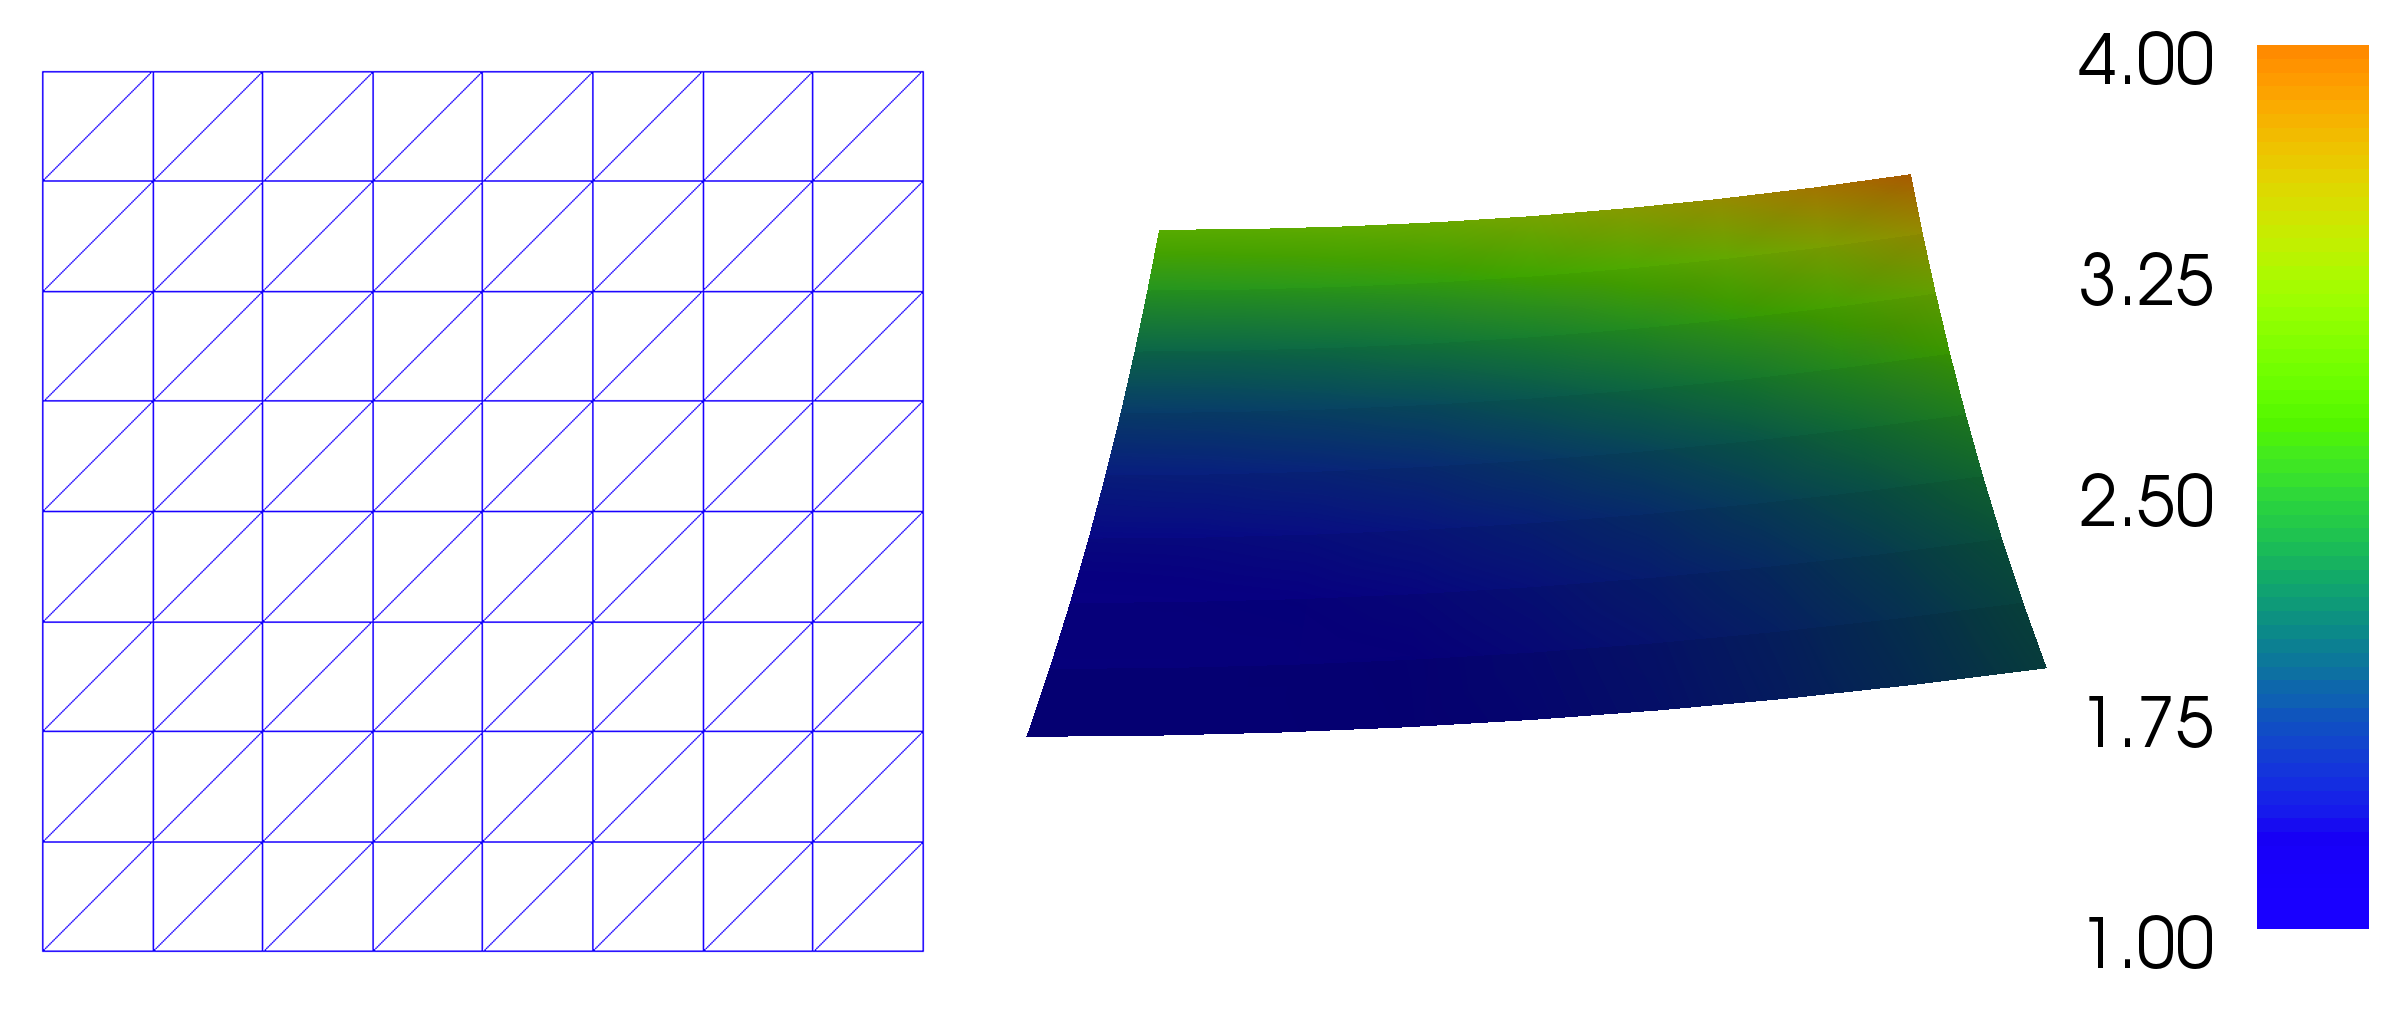
\includegraphics[width=0.95\linewidth]{fig/poisson_plot.png}}
%  \caption{
%  Plot of the mesh and the solution for the Poisson problem created using the built-in FEniCS visualization tool (\texttt{plot} command). \label{fig:poisson_plot}
%  }
%\end{figure}

\texttt{plot}命令对调试和初步科学有用
调查。 更高级的可视化更好地创建
将解决方案导出到文件并使用高级可视化
像ParaView这样的工具,如下一节所述。

通过在绘图窗口中单击鼠标左键,您可以旋转
解决方案,而鼠标右键用于缩放。 点
鼠标到\texttt{Help}文本左下角显示一个
列出所有可用的快捷命令。 帮助菜单可能
或者通过在绘图窗口中键入\textbf{h}来激活。该
\texttt{plot}命令也接受一些额外的参数,如
例如设置绘图窗口的标题:

\begin{python}
plot(u, title='Finite element solution')
plot(mesh, title='Finite element mesh')
\end{python}

有关详细的文档,请运行命令\texttt{help(plot)}
Python或\texttt{pydoc fenics.plot}从终端窗口。

\begin{notice}[Mac OS X和Docker内置绘图]
FEniCS中的内置绘图可能无法按预期方式工作
在Mac OS X上运行或在FEniCS Docker容器内运行时。
FEniCS支持使用Mac OS X上的\texttt{plot}命令进行绘图
但是,键盘快捷键可能会失败
上班。 当在Docker容器内运行时,绘图不是
因为Docker不与您的窗口系统进行交互。
对于需要绘图的Docker用户,建议您进行任何工作
在Jupyter/FEniCS notebook中(命令\texttt{fenicsproject notebook})
或依靠ParaView或其他外部工具进行可视化。
\end{notice}

\subsection{使用ParaView绘制解决方案}

\index{exporting solutions}
\index{postprocessing}
\index{ParaView}

简单的\texttt{plot}命令对于快速可视化是有用的,但是对于
更高级的可视化必须使用外部工具。 在这个
我们演示如何在ParaView中可视化解决方案。
\begin{center}
  \url{http://www.paraview.org}\footnote{\texttt{http://www.paraview.org}}
\end{center}
Paraview是一个强大的
用于可视化标量和矢量场的工具,包括那些
由FEniCS计算。

第一步是以VTK格式导出解决方案:

\begin{python}
vtkfile = File('poisson/solution.pvd')
vtkfile << u
\end{python}

以下步骤演示如何创建解决方案
我们在ParaView中的Poisson问题。 得到的情节显示在
Figure~\ref{fig:poisson_paraview}。

\begin{enumerate}
\item 启动ParaView应用程序。

\item 单击顶部菜单中的\textbf{File--Open...},导航到包含导出解决方案的目录。 这应该在FEniCS Python程序启动目录下面的名为\texttt{poisson}的子目录中。 选择文件\texttt{solution.pvd},然后单击\textbf{OK}。

\item 在左侧的Properties窗格中单击\textbf{Apply}。 这将提出解决方案。

\item 要制作解决方案的3D图,我们将使用ParaView的许多\emph{filters}之一。 单击顶部菜单中的\textbf{Filters--Alphabetical--Warp By Scalar},然后在左侧的Properties窗格中单击\textbf{Apply}。 这产生了由解值确定的高度的高架表面。

\item 要在升高的表面下显示原始图表,请单击左侧Pipeline浏览器窗格中\texttt{solution.pvd}左侧的小眼图标。 还可以点击绘图窗口顶部的小2D按钮,将可视化文件更改为3D。 这可以通过旋转 (鼠标左键) 和缩放 (Ctrl +鼠标左键) 与图形交互。

\item 要显示有限元网格,请在Pipeline浏览器中单击\texttt{solution.pvd},导航到Properties窗格中的\textbf{Representation},然后选择\textbf{Surface With Edges}。 这应该使有限元网格可见。

\item 要更改绘图的宽高比,请单击Pipeline浏览器中的\textbf{WarpByScalar1},然后导航到Properties窗格中的\textbf{Scale Factor}。 将值更改为0.2,然后单击\textbf{Apply}。 这将改变扭曲情节的规模。 我们还在Properties窗格的底部单击\textbf{Orientation Axis Visibility},以删除绘图窗口左下角的小3D轴。 你现在应该看到类似于Figure~\ref{fig:poisson_paraview}的情节。

\item 最后,要将可视化文件导出到文件中,请单击\textbf{File--Save Screenshot...},然后选择一个合适的文件名,如\texttt{poisson.png}。
\end{enumerate}

\noindent
有关更多信息,请参阅ParaView指南\cite{Paraview}
(免费PDF可用),
\begin{center}
  \url{http://www.paraview.org/Wiki/The_ParaView_Tutorial} {ParaView tutorial} \footnote{\texttt{http://www.paraview.org/Wiki/The\_ParaView\_Tutorial}}
\end{center}
  和指令video
\begin{center}
  \url{https://vimeo.com/34037236} {ParaView简介} \footnote{\texttt{https://vimeo.com/34037236}}。
\end{center}

%\begin{figure}[!ht]  % fig:poisson_paraview
%  \centerline{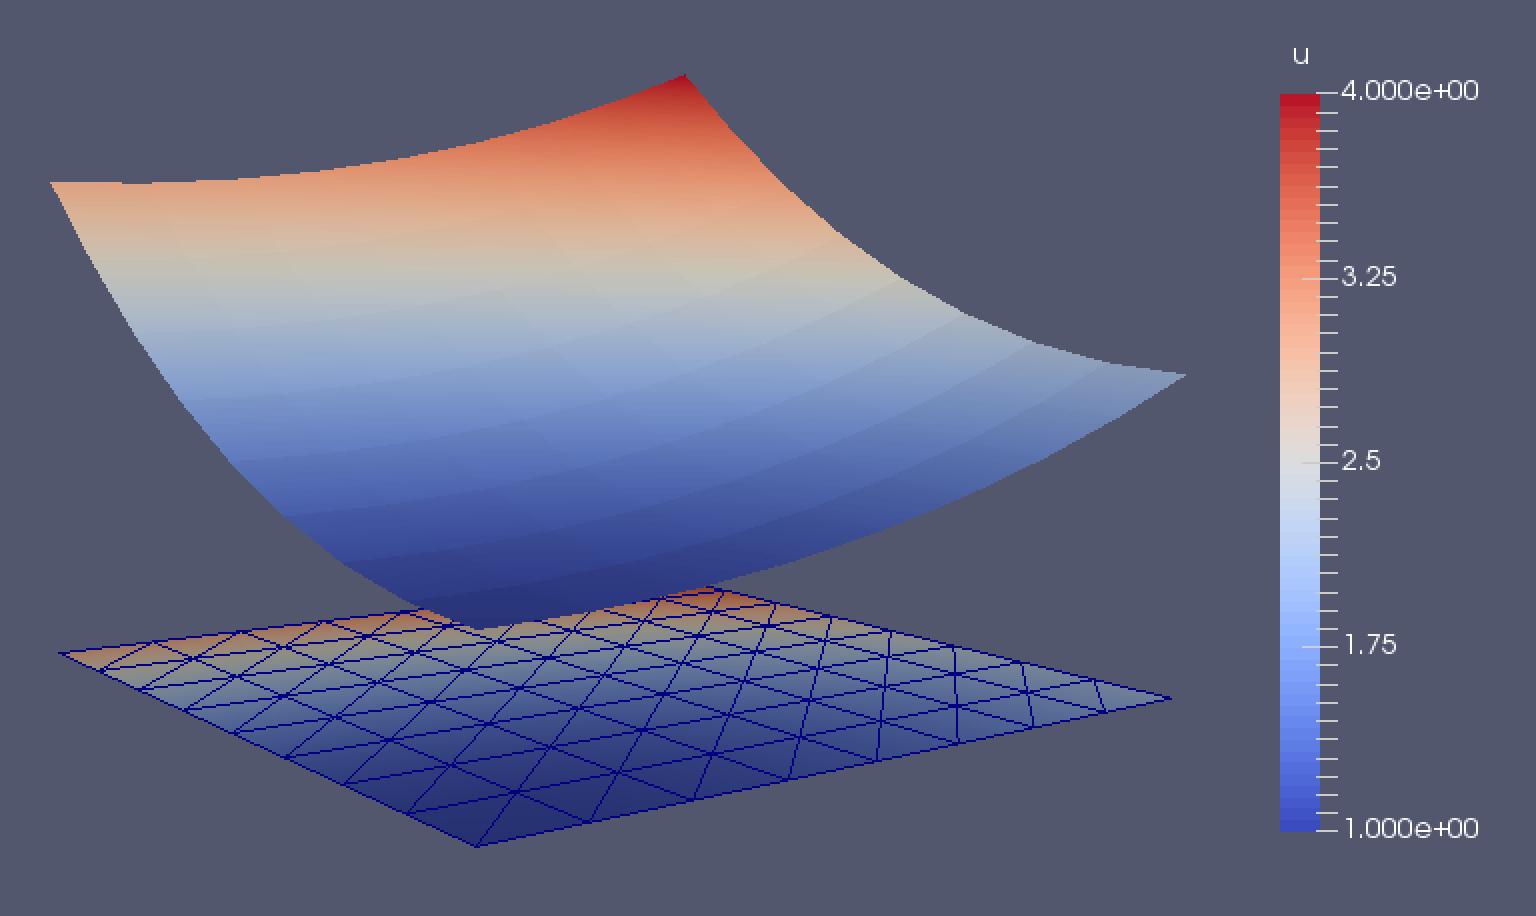
\includegraphics[width=0.95\linewidth]{fig/poisson_paraview.png}}
%  \caption{
%  Plot of the mesh and the solution for the Poisson problem created using ParaView. \label{fig:poisson_paraview}
%  }
%\end{figure}

\subsection{计算错误}

\index{error}

最后,我们计算错误以检查解决方案的准确性。
我们通过将有限元解决方案\texttt{u}与确切的比较来做到这一点
解决方案,在这个例子中恰好与之相同
表达\verb!u_D! 用于设置边界条件。 我们计算
错误有两种不同的方式。 首先,我们计算$L^2$ norm
错误,由...定义

\[ E = \sqrt{\int_\Omega (\ub - u)^2\dx}\tp\]
由于确切的解是二次方程和有限元解
是分段线性的,这个错误将是非零。 计算此错误
在FEniCS中,我们简单地写道

\begin{python}
error_L2 = errornorm(u_D, u, 'L2')
\end{python}
\texttt{errornorm}函数也可以计算其他错误规范
作为$H^1$标准。 在终端窗口中键入\texttt{pydoc fenics.errornorm}
详细信息。

我们还计算所有顶点的误差的最大值
有限元网格。 如上所述,我们期待这个错误
对于该特定示例,对于机器内部的精度为零。 至
计算顶点的误差,我们先要求FEniCS来计算
两个\verb!u_D!的值 和\texttt{u}在所有顶点,然后减去
结果:

\begin{python}
vertex_values_u_D = u_D.compute_vertex_values(mesh)
vertex_values_u = u.compute_vertex_values(mesh)
import numpy as np
error_max = np.max(np.abs(vertex_values_u_D - vertex_values_u))
\end{python}
我们在这里使用\texttt{numpy}的最大和绝对值函数,
因为这些对于大型阵列(因子为30)要高得多,
比Python的内置\texttt{max}和\texttt{abs}函数。

\begin{notice}[如何检查错误消失]
用不精确(浮点)算术,最大
顶点的错误不是零,而应该是一个小数字。该
机器精度约为$10^{-16}$,但在有限元中
计算,这个大小的舍入误差可能会累积,产生
大于$10^{-16}$的错误。 实验表明,增加
元素数量增加有限元的程度
多项式增加误差。 对于一个网格
$2\times(20\times20)$ cubic xxxLagrange元素(3级),错误大约是$2\cdot
10^{-12}$,而对于128个线性元素,错误大约是$2\cdot
10^{-15}$。
\end{notice}

\subsection{检查自由度和顶点值}
\label{ch:poisson0:impl:dofmap}

\index{degrees of freedom}
\index{vertex values}
\index{nodal values}
\index{dofs}

有限元函数(如$u$)表示为线性组合
的基础函数$\phi_j$,跨越空间$V$:

\begin{equation}
u = \sum_{j=1}^N U_j \phi_j \label{ch:poisson0:ufem}\tp
\end{equation}

通过在程序中写入\texttt{solve(a == L,u,bc)},线性系统将会
由$a$和$L$组成,这个系统是为了解决的
值$U_1,\ldots,U_N$。 值$U_1,\ldots,U_N$被称为
\emph{degree of freedom}(``dofs'')或\emph{nodal values}为$u$。 对于Lagrange
元素(和许多其他元素类型)$U_j$只是它的值
$u$在全局号为$j$的节点上。 节点的位置和
对于线性的Lagrange元素,单元格顶点重合,而for
高阶元素有与之相关联的附加节点
小平面,边缘,有时也是细胞的内部。

将\texttt{u}表示为\texttt{Function}对象,我们可以进行评估
\texttt{u(x)}在网格中的任何点\texttt{x}(昂贵的操作!),或者我们可以
在矢量$U$中直接获取所有自由度

\begin{python}
nodal_values_u = u.vector()
\end{python}
结果是一个\texttt{Vector}对象,它基本上是一个封装
在使用的线性代数包中使用的矢量对象
解决变分问题引起的线性系统。
由于我们在Python中编程,所以转换\texttt{Vector}
对象到标准\texttt{numpy}数组进行进一步处理:

\index{degrees of freedom}
\index{nodal values}
\index{numbering!degrees of freedom}
\index{numbering!cell vertices}

\begin{python}
array_u = nodal_values_u.array()
\end{python}

使用\texttt{numpy}数组,我们可以编写类似MATLAB的代码来分析
数据。 索引用方括号完成:\verb!array_u [j]!,其中
index \texttt{j}始终从\texttt{0}开始。 如果解决方案是用
分段线性Lagrange元素($\mathsf{P}_1$),然后是大小
数组\verb!array_u! 等于顶点的数量,每个
\verb!array_u[J]! 是网格中某个顶点的值。 但是,学位
的自由并不一定按照相同的方式编号
的顶点
目。 (这在〜\ref{ch:poisson0:verify1}部分中有详细的讨论)。
如果我们想要知道顶点的值,我们需要
调用函数\verb!u.compute_vertex_values! 此函数返回
网格的所有顶点的值与\texttt{numpy}数组相同
对于网格的顶点编号,例如:

\begin{python}
vertex_values_u = u.compute_vertex_values()
\end{python}

请注意,对于$\mathsf{P}_1$元素, \verb!array_u! 和\verb!vertex_values_u! 具有相同的长度并且包含相同的值,尽管以不同的顺序。
